% =============================================================================
%  The Mathematics of Virtual Colonoscopy · Flagship Lecture (v2, council-revised)
%  Flattening the Colon: from "why you can't" to one method you compute by hand
%  Mode: passive-study · theme: teal · ONE driving question, depth over breadth.
%  Design: 5-question spine; every concept earned by a question; every climax computed.
%  Honest scope: builds the discrete HARMONIC map (fixed boundary) ~ conformal.
%  Prose: en-technical-style. Rigor: rigor-and-citations (prove special case / cite + verified links).
%  Figures: openly-licensed only (CC0), credited. No copyrighted paper figures.
% =============================================================================
\documentclass[aspectratio=169,10pt]{beamer}
\usepackage[teal]{template-lib/template-lib}
\uselayout{text}
\uselayout{eq}
\uselayout{twocol}

\usetikzlibrary{arrows.meta,calc,positioning,patterns,decorations.pathmorphing,%
  decorations.markings,shapes.geometric,backgrounds}

\newcommand{\R}{\mathbb{R}}
\newcommand{\grad}{\nabla}
\newcommand{\Lap}{\Delta}
\newcommand{\half}{\tfrac{1}{2}}
\newcommand{\inner}[2]{\langle #1,#2\rangle}
\newcommand{\nm}[1]{\lVert #1\rVert}
\newcommand{\xb}{\mathbf{x}}
\newcommand{\Lmat}{\mathbf{L}}
\newcommand{\dd}{\mathrm{d}}

\TLsetfoot{Flattening the Colon \textperiodcentered{} from ``why you can't'' to one method you compute by hand}

\begin{document}

% =============================================================================
\TLtitlecenter
  {Flattening the Colon}
  {From ``why you can't'' to one method you can compute by hand}
  {The Mathematics of Virtual Colonoscopy \textperiodcentered{} Flagship Lecture (I)}
  {Self-study lecture · build it, don't memorize it}

% =============================================================================
\begin{frame}{How to read this lecture}
  One question drives the whole deck:
  \begin{center}
    \emph{Can we lay a curved colon flat so a doctor sees every patch --- without\\
    lying about a polyp's shape? If not perfectly, how close, and how?}
  \end{center}
  The contract for a self-study deck:
  \begin{itemize}
    \item \textbf{Every concept is earned by a question} --- nothing named before you need it.
    \item \textbf{Every claim that matters is computed}, so you can re-derive it with pencil.
    \item We build \textbf{one} method end to end; deeper methods are named at the end as the next decks.
    \item Prerequisites: calculus and linear algebra. \emph{No} differential geometry, \emph{no} complex analysis.
  \end{itemize}
  \TLtakeaway{Goal: finish able to flatten a small mesh \emph{by hand}, and say exactly what it keeps, what it costs, and why the cost is unavoidable.}
\end{frame}

% =============================================================================
\begin{frame}{The five questions (the whole deck on one page)}
  \begin{enumerate}
    \item[\textbf{Q1}] I cut the colon open and pressed it flat --- \textbf{what broke?} \hfill (the \emph{metric})
    \item[\textbf{Q2}] When can the metric be made flat at all? \hfill (\emph{curvature}; why you can't)
    \item[\textbf{Q3}] Forced to distort, what is the least-bad thing to keep? \hfill (\emph{conformal}: keep angles)
    \item[\textbf{Q4}] How do we actually compute it on a real (mesh) colon? \hfill (the \emph{cotangent Laplacian})
    \item[\textbf{Q5}] Did it work, and what did we pay? \hfill (measure it; close the loop)
  \end{enumerate}
  \TLtakeaway{Each question forces the next concept. Q2 is a clean ``no''; Q3--Q5 build and audit the least-bad alternative.}
\end{frame}

% =============================================================================
\TLsection{Q1 · I cut it open and pressed it flat --- what broke?}

% --- 1.1 the failed experiment ----------------------------------------------
\begin{frame}{A failed experiment}
  \begin{columns}[T]
    \begin{column}{0.55\textwidth}
      Try the obvious thing. Cut the colon (a tube) along one line and press it onto a table.
      \begin{itemize}
        \item Paint a small triangle on the wall; measure its three edge lengths \emph{on the surface}.
        \item Measure the same edges \emph{after} pressing flat. They \textbf{differ} --- some stretched, some squeezed.
      \end{itemize}
      The organizing question: \emph{what would have been preserved if the flattening were honest?} Whatever it is, we need to measure length \emph{using the surface itself}.
    \end{column}
    \begin{column}{0.45\textwidth}
      \centering
      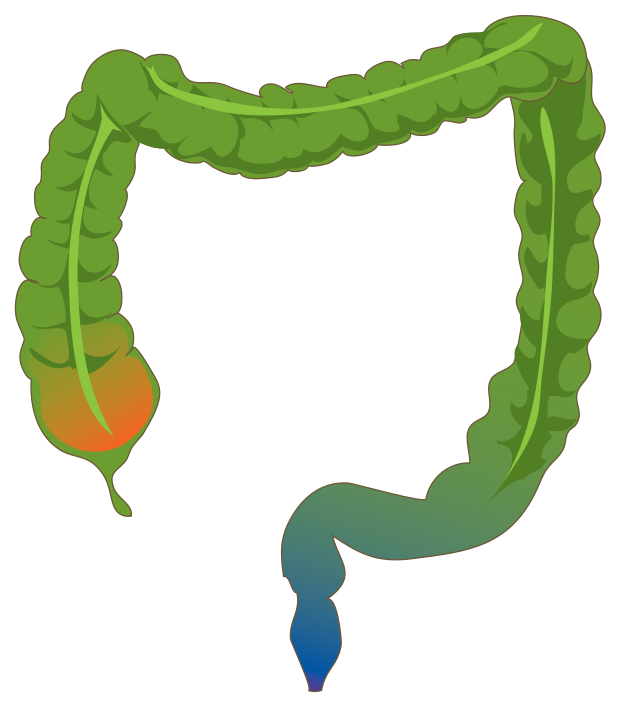
\includegraphics[height=3.5cm]{assets/colon-en/colon_anatomy.png}\\[2pt]
      {\scriptsize The colon: a tube we cut open and press flat.\\
       Figure: Mikael Häggström, \href{https://commons.wikimedia.org/wiki/File:Colon_(anatomy).svg}{Wikimedia Commons}, public domain.}
    \end{column}
  \end{columns}
  \TLtakeaway{``Flatten without distortion'' must mean: \emph{preserve the lengths the surface itself measures.} So first we need that measuring device.}
\end{frame}

% --- 1.2 surfaces 101 -------------------------------------------------------
\begin{frame}{A surface is a map; its tangent vectors do the measuring}
  Write a surface as a map from a flat parameter region into space:
  \[
    \xb(u,v)\in\R^3,\qquad (u,v)\in\Omega\subset\R^2 .
  \]
  \begin{columns}[T]
    \begin{column}{0.6\textwidth}
      \begin{itemize}
        \item The \textbf{tangent vectors} $\xb_u=\partial\xb/\partial u,\ \xb_v=\partial\xb/\partial v$ span the tangent plane.
        \item A small step $(\dd u,\dd v)$ moves you in 3D by $\dd\xb=\xb_u\,\dd u+\xb_v\,\dd v$, of length $\nm{\dd\xb}$.
      \end{itemize}
      Everything we measure on the surface hides in the three dot products of $\xb_u,\xb_v$.
    \end{column}
    \begin{column}{0.4\textwidth}
      \centering
      \begin{tikzpicture}[scale=0.8,every node/.style={font=\scriptsize}]
        \draw[gray!50] (-1.6,-0.2) rectangle (-0.2,1.0);
        \node[gray] at (-0.9,-0.5) {$(u,v)$ chart};
        \fill (-1.1,0.4) circle (1pt);
        \draw[->,>=Stealth] (1.2,1.4)--(1.2,1.0);
        \draw[TLprimary,thick] (0.4,0.1) .. controls (1.2,0.7) and (2.0,0.5) .. (2.6,1.0);
        \draw[TLprimary,thick] (0.4,0.1) .. controls (0.7,0.7) and (0.9,1.1) .. (1.1,1.7);
        \fill (0.9,0.55) circle (1pt) node[below right,black]{$\xb(u,v)$};
        \draw[->,TLaccent,thick] (0.9,0.55)--(1.7,0.75) node[right,black]{$\xb_u$};
        \draw[->,TLneg,thick] (0.9,0.55)--(1.05,1.25) node[above,black]{$\xb_v$};
      \end{tikzpicture}
    \end{column}
  \end{columns}
  \TLtakeaway{A surface point is $\xb(u,v)$; the tangent vectors $\xb_u,\xb_v$ are the rulers. Next: turn them into one length-and-angle formula.}
\end{frame}

% --- 1.3 the metric, born computed ------------------------------------------
\begin{frame}{The metric (first fundamental form) --- born as dot products}
  Square the step $\dd\xb=\xb_u\,\dd u+\xb_v\,\dd v$:
  \[
    \nm{\dd\xb}^2=\underbrace{\inner{\xb_u}{\xb_u}}_{E}\dd u^2+2\underbrace{\inner{\xb_u}{\xb_v}}_{F}\dd u\,\dd v+\underbrace{\inner{\xb_v}{\xb_v}}_{G}\dd v^2 .
  \]
  The three numbers $E,F,G$ are the \TLterm{first fundamental form} (the \TLterm{metric}). They are all you need to measure on the surface:
  \begin{itemize}
    \item \textbf{length} of any curve (integrate $\nm{\dd\xb}$), and \textbf{angle} between two steps (via $\inner{\cdot}{\cdot}$ built from $E,F,G$).
    \item ``Flatten without distortion'' now has a precise meaning: a map to the plane that leaves $E,F,G$ unchanged --- an \TLterm{isometry}.
  \end{itemize}
  \TLtakeaway{The metric is just $\inner{\xb_u}{\xb_u},\inner{\xb_u}{\xb_v},\inner{\xb_v}{\xb_v}$. ``Distortion-free'' $=$ ``same metric.'' Let's compute it for the two shapes that decide our problem.}
\end{frame}

% --- 1.4 cylinder metric ----------------------------------------------------
\begin{frame}{The cylinder's metric is secretly the flat plane's}
  Parametrize a radius-$r$ cylinder: $\xb(u,v)=(r\cos u,\;r\sin u,\;v)$.
  \[
    \xb_u=(-r\sin u,\;r\cos u,\;0),\quad \xb_v=(0,0,1)
    \ \Rightarrow\ E=r^2,\ F=0,\ G=1 .
  \]
  Rescale the angular coordinate, $\tilde u=r u$. Then $\dd\xb$ has
  \[
    \nm{\dd\xb}^2=\dd\tilde u^2+\dd v^2 \quad(\text{exactly the plane's metric}).
  \]
  \TLresultblock{So the cylinder unrolls with zero distortion}{In the $(\tilde u,v)$ coordinates the metric is the identity --- the same as flat paper. The cylinder \emph{is} flat paper, rolled up. You can press it onto a table without stretching anything --- \textbf{after one cut} (a tube is a loop; cut it to a strip).}
  \TLtakeaway{The colon is a tube too --- so we will cut it open. If the colon were a perfect cylinder we would be done. It isn't, and the next slide shows why.}
\end{frame}

% --- 1.5 sphere metric + bridge ---------------------------------------------
\begin{frame}{The sphere's metric refuses to go flat}
  \begin{columns}[T]
    \begin{column}{0.58\textwidth}
      A radius-$R$ sphere: $\xb(\phi,\theta)=(R\sin\phi\cos\theta,\,R\sin\phi\sin\theta,\,R\cos\phi)$.
      \[
        E=R^2,\quad F=0,\quad G=R^2\sin^2\phi .
      \]
      The factor $\sin^2\phi$ depends on \emph{where} you are, and no rescaling removes it the way $\tilde u=ru$ fixed the cylinder. The sphere's metric is \emph{not} the flat metric in disguise.
      \begin{itemize}
        \item Cylinder: metric can be made flat $\Rightarrow$ unrolls perfectly.
        \item Sphere: it cannot $\Rightarrow$ (we suspect) it cannot be flattened.
      \end{itemize}
    \end{column}
    \begin{column}{0.42\textwidth}
      \TLwarnblock{The real question}{What is the \emph{obstruction}? Some shapes' metrics can be made flat (cylinder) and some can't (sphere). There must be a single quantity, computable from $E,F,G$ alone, that decides. Finding it is Q2.}
    \end{column}
  \end{columns}
  \TLtakeaway{The colon is mostly cylinder-like but its haustral folds bend it like little spheres --- so we expect it to sit on the ``can't'' side. Q2 makes ``can't'' precise and proves it.}
\end{frame}

% =============================================================================
\TLsection{Q2 · When can the metric be made flat? The obstruction is curvature}

% --- 2.1 principal curvatures -----------------------------------------------
\begin{frame}{One number for how a surface bends}
  At a point, slice the surface by planes through the normal and read how sharply each slice curves. The extremes are the \TLterm{principal curvatures} $\kappa_1,\kappa_2$.
  \begin{columns}[T]
    \begin{column}{0.56\textwidth}
      \begin{itemize}
        \item \textbf{Cylinder} (radius $r$): bends one way, flat the other $\Rightarrow \kappa_1=\tfrac1r,\ \kappa_2=0$.
        \item \textbf{Sphere} (radius $R$): bends equally every way $\Rightarrow \kappa_1=\kappa_2=\tfrac1R$.
      \end{itemize}
      We want a \emph{single} number, and it should already know that the cylinder is special.
    \end{column}
    \begin{column}{0.44\textwidth}
      \centering
      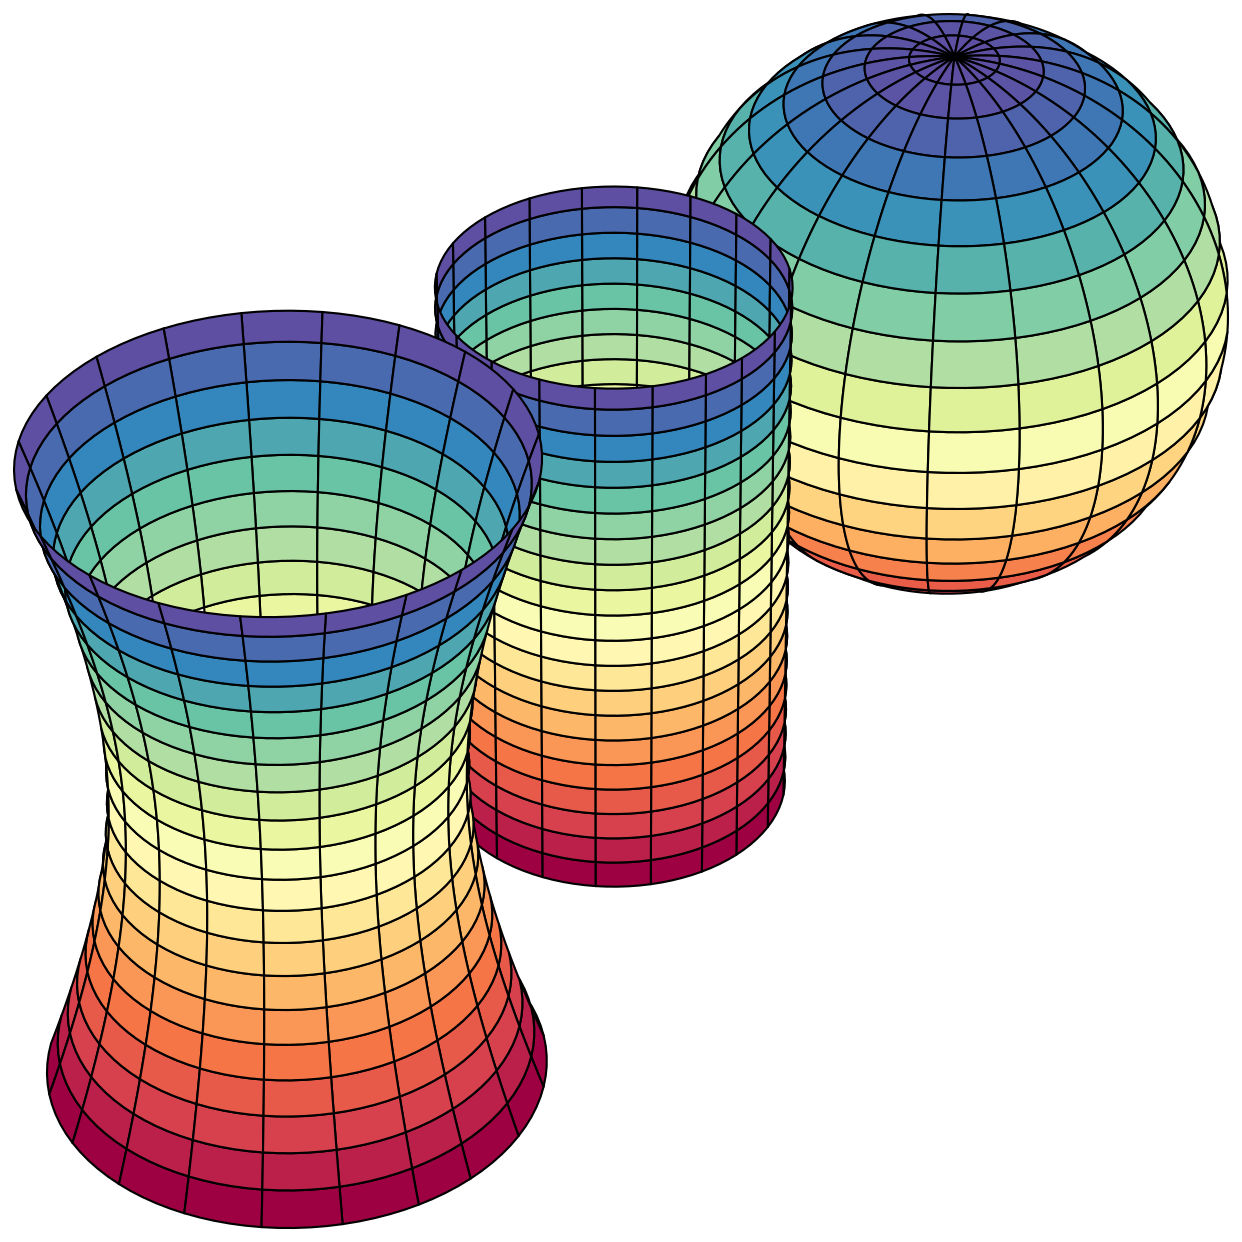
\includegraphics[height=2.7cm]{assets/colon-en/gaussian_curvature.png}\\[2pt]
      {\scriptsize $K\!<\!0$ saddle \textperiodcentered\ $K\!=\!0$ cylinder \textperiodcentered\ $K\!>\!0$ sphere.\\
       Figure: Nicoguaro, \href{https://commons.wikimedia.org/wiki/File:Gaussian_curvature.svg}{Wikimedia Commons}, CC0.}
    \end{column}
  \end{columns}
  \TLtakeaway{The product $\kappa_1\kappa_2$ is the candidate: it is $0$ for the cylinder (one factor vanishes) and nonzero for the sphere. That product is Gauss curvature.}
\end{frame}

% --- 2.2 Gauss curvature ----------------------------------------------------
\begin{frame}{Gauss curvature $K=\kappa_1\kappa_2$, computed}
  \[
    \boxed{\,K=\kappa_1\kappa_2\,}\qquad\Longrightarrow\qquad
    K_{\text{cylinder}}=\tfrac1r\cdot 0=0,\qquad
    K_{\text{sphere}}=\tfrac1R\cdot\tfrac1R=\tfrac{1}{R^2}.
  \]
  \begin{itemize}
    \item The cylinder ($K=0$) is exactly the shape that unrolled. The sphere ($K\neq0$) is the one whose metric refused to go flat.
    \item \textbf{Conjecture}: $K$ is the obstruction --- a surface can be flattened without distortion only where $K=0$.
  \end{itemize}
  But there is a catch that makes this look hopeless: $\kappa_1,\kappa_2$ describe how the surface bends \emph{in space} (extrinsic). An in-surface ant, who only knows $E,F,G$, seems unable to know $K$. The next slide is the miracle that saves the conjecture.
  \TLtakeaway{$K$ separates ``flattenable'' (cylinder, $K{=}0$) from ``not'' (sphere, $K{\neq}0$). To make it a theorem we need $K$ to be measurable from the metric alone.}
\end{frame}

% --- 2.3 Theorema Egregium --------------------------------------------------
\begin{frame}{Gauss's miracle: $K$ is intrinsic (Theorema Egregium)}
  \TLresultblock{Theorema Egregium (Gauss, 1827)}{Although $K=\kappa_1\kappa_2$ is \emph{defined} from how the surface bends in space, it is in fact computable from the metric $E,F,G$ and their derivatives \emph{alone}. So $K$ is \TLterm{intrinsic}: an in-surface ant can measure it.}
  \medskip
  The consequence we need: an \textbf{isometry preserves the metric, hence preserves $K$}.
  \begin{itemize}
    \item We only use the \emph{easy} direction: $K\neq0$ somewhere $\Rightarrow$ no isometric flattening there. (The converse ``$K\equiv0\Rightarrow$ locally flat'' is Minding's theorem --- cited, not needed.)
  \end{itemize}
  \TLinfoblock{Full proof (cited, not sketched)}{The general proof (Brioschi's formula) is $\sim$2 pages: see \href{https://en.wikipedia.org/wiki/Theorema_Egregium}{Theorema Egregium} and do~Carmo, \emph{Diff.\ Geometry of Curves \& Surfaces}, \S4-3. We take $K$'s intrinsic-ness as given; what we \emph{do} prove, in full, is the impossibility it implies (next slide).}
\end{frame}

% --- 2.4 impossibility proven -----------------------------------------------
\begin{frame}{The impossibility, proven}
  \begin{columns}[T]
    \begin{column}{0.58\textwidth}
      Suppose an isometric flattening $\phi:S\to\text{plane}$ existed. Then:
      \begin{enumerate}
        \item $\phi$ is an isometry $\Rightarrow$ it preserves the metric $\Rightarrow$ (Theorema Egregium) it preserves $K$ at corresponding points.
        \item The plane has $K=0$ everywhere.
        \item Therefore $K_S=0$ at every point of $S$.
        \item But the colon's folds bend it two ways, so $K_S\neq0$ on a patch of positive area.
      \end{enumerate}
      Steps 3 and 4 contradict. So $\phi$ cannot exist.
    \end{column}
    \begin{column}{0.42\textwidth}
      \TLresultblock{No distortion-free flattening}{$K\neq0$ somewhere on the colon $\;\Longrightarrow\;$ \textbf{no isometric map to the plane exists.} You cannot keep all lengths. Full stop.}
    \end{column}
  \end{columns}
  \TLtakeaway{This is a clean \emph{no}, and it is the design constraint for the rest of the lecture: we must give something up. Q3 asks --- give up \emph{what}?}
\end{frame}

% =============================================================================
\TLsection{Q3 · Isometry is dead. Why keep angles?}

% --- 3.1 the choice (weakest-link fix) --------------------------------------
\begin{frame}{Three things a flattening could keep --- pick one}
  A map to the plane can try to preserve \textbf{length}, \textbf{angle}, or \textbf{area}. Length is impossible (Q2). Between angle and area, which serves the doctor?
  \begin{columns}[T]
    \begin{column}{0.54\textwidth}
      \TLinfoblock{Keep angles (conformal)}{A polyp is spotted by its \emph{round shape}. A map that preserves angles sends round things to round things, so the radiologist's shape-based read survives the flattening.}
    \end{column}
    \begin{column}{0.46\textwidth}
      \TLwarnblock{Keep area instead?}{Area-preserving maps shear shapes --- a round polyp becomes an ellipse, the one cue the doctor relies on. And area error is a single global factor you can color-code and annotate.}
    \end{column}
  \end{columns}
  \medskip
  So we keep \textbf{angles} and pay in \textbf{area}. A map that preserves angles is called \TLterm{conformal}.
  \TLtakeaway{The clinical reason --- keep shapes legible --- is what forces angle-preservation over area-preservation. It is not an arbitrary mathematical taste.}
\end{frame}

% --- 3.2 conformal defined + shown ------------------------------------------
\begin{frame}{Conformal $=$ scale the metric by one positive factor}
  \TLterm{Conformal map}: the pulled-back metric is the original times a positive scalar field,
  \[
    \phi^{*}g_{\text{plane}}=e^{2u}\,g,\qquad e^{2u}>0\ \text{the \TLterm{conformal factor}}.
  \]
  Why this keeps angles but charges area --- a three-line check. Scale $g\mapsto e^{2u}g$:
  \[
    \cos\angle=\frac{\inner{a}{b}_{e^{2u}g}}{\nm{a}_{e^{2u}g}\,\nm{b}_{e^{2u}g}}
    =\frac{e^{2u}\inner{a}{b}_g}{e^{u}\nm{a}_g\cdot e^{u}\nm{b}_g}
    =\frac{\inner{a}{b}_g}{\nm{a}_g\nm{b}_g}\quad(\textbf{angle unchanged}),
  \]
  while the area element $\dd A=\sqrt{\det g}\,\dd u\,\dd v$ becomes $\sqrt{\det(e^{2u}g)}=e^{2u}\sqrt{\det g}$ (\textbf{area} $\times e^{2u}$).
  \TLtakeaway{The single factor $e^{2u}$ cancels in the angle ratio but multiplies the area. Angles free; area is the whole bill. This is exactly the trade we wanted.}
\end{frame}

% --- 3.3 circle stays circle + concrete number ------------------------------
\begin{frame}{Picture and a number: circles stay circles}
  \begin{columns}[T]
    \begin{column}{0.56\textwidth}
      Because the scaling is the \emph{same in every direction}, the map's Jacobian is $e^{u}\times(\text{rotation})$. So an infinitesimal circle maps to an infinitesimal \emph{circle} --- resized, never sheared into an ellipse.
      \medskip
      A concrete factor: stereographic projection of the radius-$1$ sphere onto the plane is conformal, with
      \[
        e^{2u}(\rho)=\frac{4}{(1+\rho^2)^2},
      \]
      where $\rho$ is the planar distance from the center. Area scale $4$ at $\rho=0$, $1$ at $\rho=1$ --- shape stays round, only size breathes.
    \end{column}
    \begin{column}{0.44\textwidth}
      \centering
      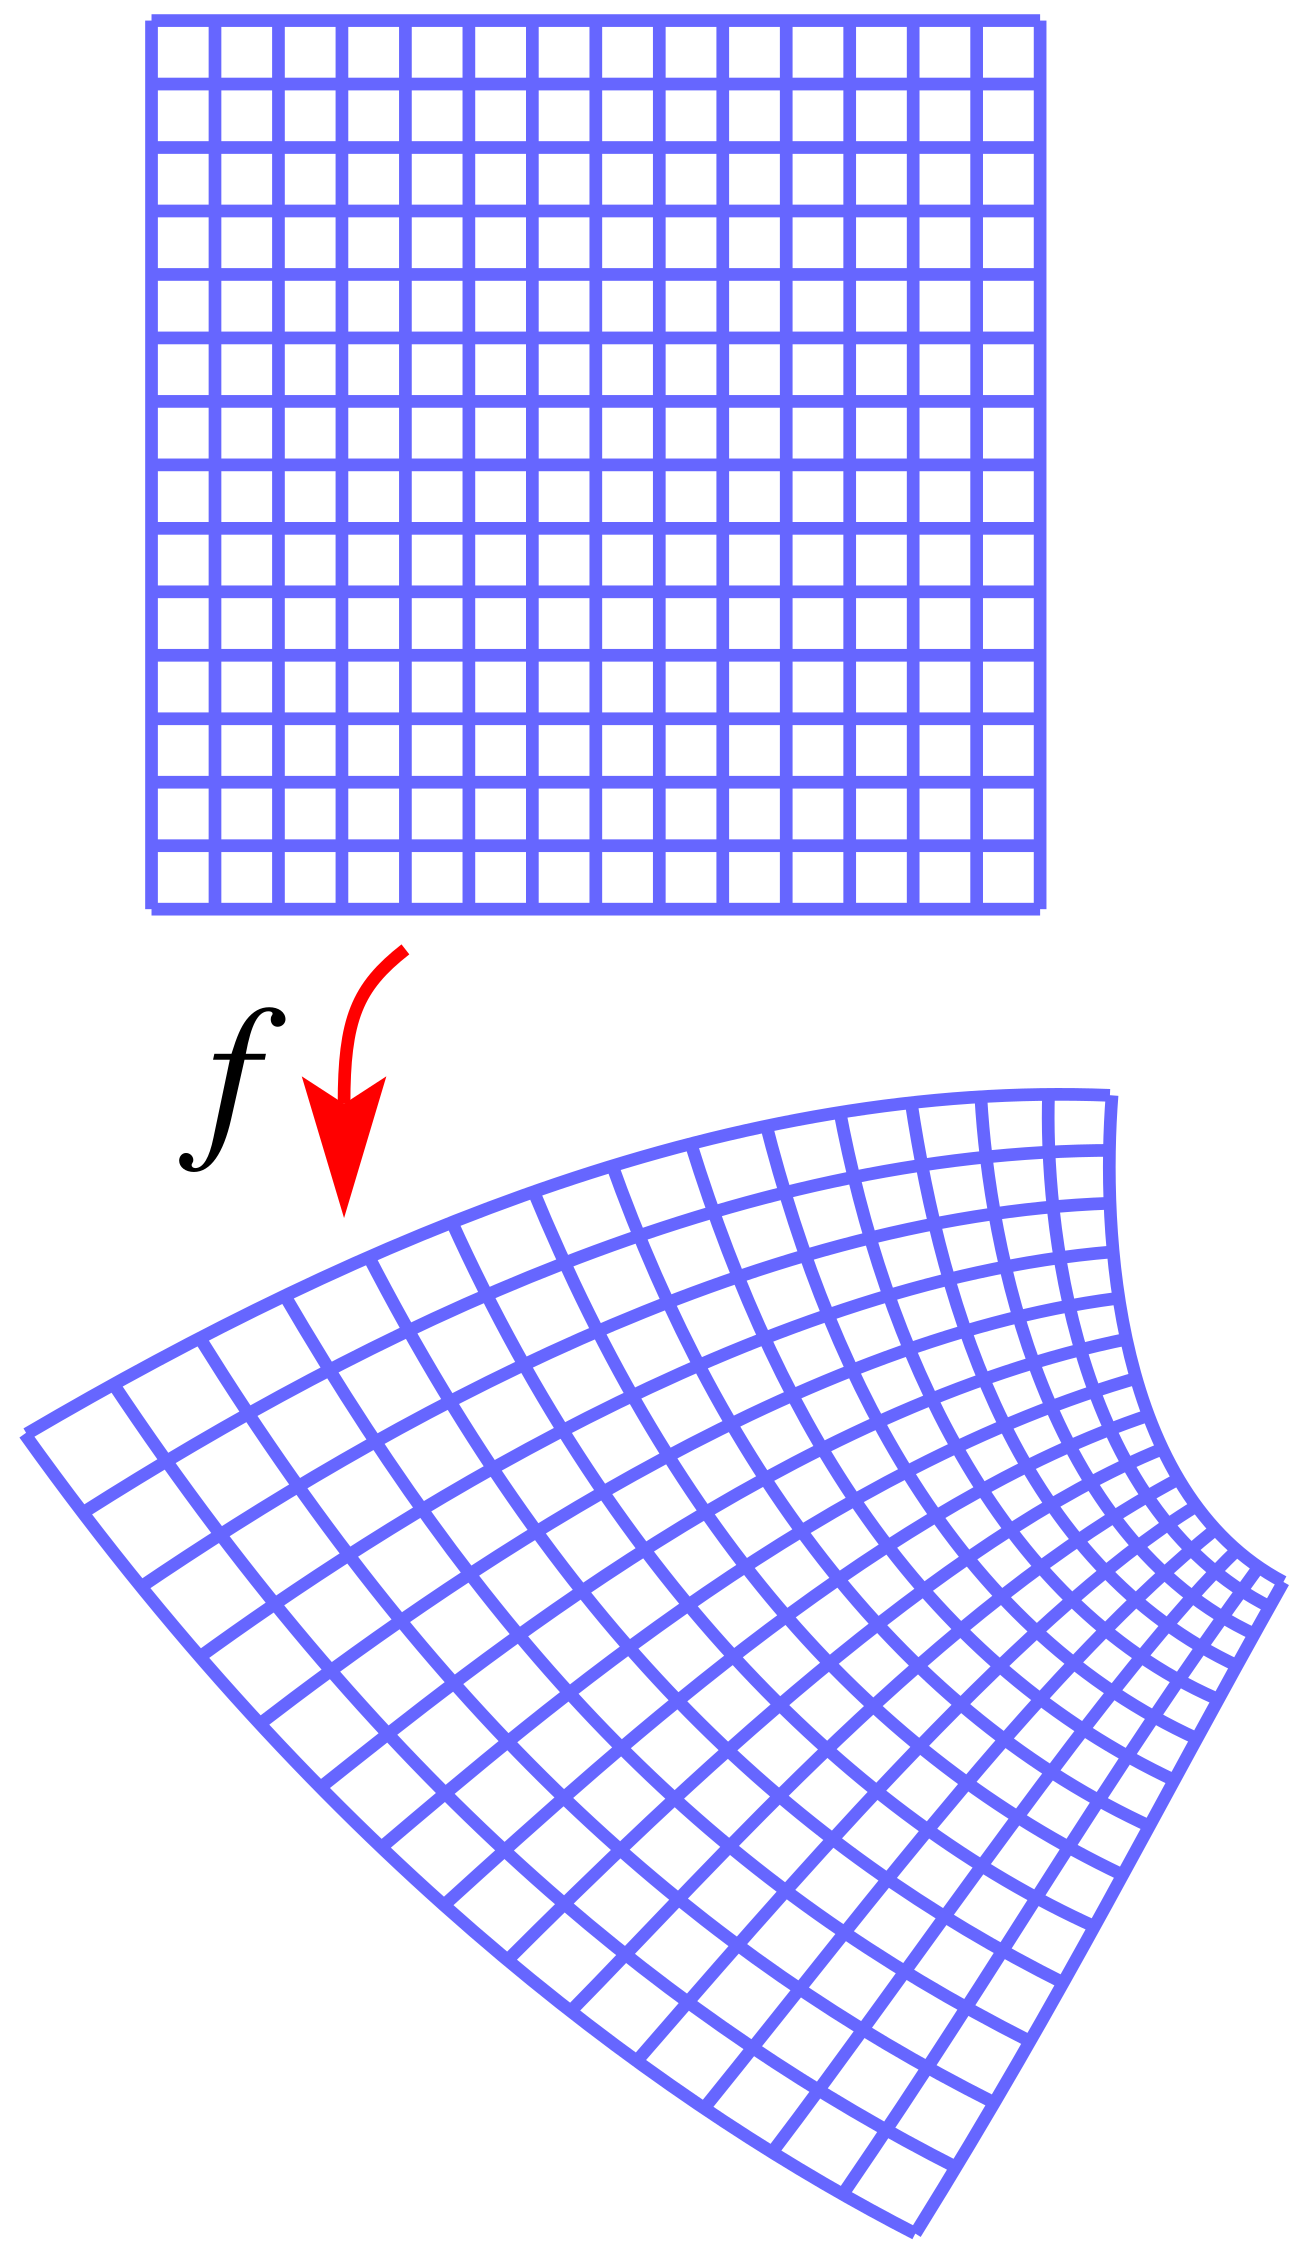
\includegraphics[height=4.0cm]{assets/colon-en/conformal_map.png}\\[2pt]
      {\scriptsize A conformal map $f$: the grid bends, yet every crossing stays a right angle.\\
       Figure: Oleg Alexandrov, \href{https://commons.wikimedia.org/wiki/File:Conformal_map.svg}{Wikimedia Commons}, public domain.}
    \end{column}
  \end{columns}
  \TLtakeaway{``Keep angles'' literally means ``keep round things round.'' The price $e^{2u}$ is now a concrete number you can read off a real map.}
\end{frame}

% --- 3.4 honesty + bridge ---------------------------------------------------
\begin{frame}{Does a conformal flattening even exist? (an honest flag)}
  \begin{columns}[T]
    \begin{column}{0.58\textwidth}
      For a \emph{smooth} colon, the statement ``a conformal map to the plane exists'' is a deep theorem --- the \href{https://en.wikipedia.org/wiki/Uniformization_theorem}{uniformization theorem}. We will \textbf{not} prove it, and we flag that honestly: in the smooth picture we take existence on faith.
      \begin{itemize}
        \item Good news: we never actually hold a smooth colon.
        \item We hold a \textbf{triangle mesh}. On a mesh the flattening is the solution of one linear system --- and \emph{existence comes free from linear algebra}, with no deep theorem.
      \end{itemize}
    \end{column}
    \begin{column}{0.42\textwidth}
      \TLinfoblock{What Q4 delivers (scope, stated up front)}{We build the discrete \emph{harmonic} map with a fixed boundary: angle-preserving in the limit, $\approx$ conformal. Making it \emph{exactly} conformal is a later deck. We are precise about this so nothing is over-claimed.}
    \end{column}
  \end{columns}
  \TLtakeaway{The discrete world sidesteps the hard existence theorem: a flattening exists because a positive-definite linear system always has a unique solution. Now build it.}
\end{frame}

% =============================================================================
\TLsection{Q4 · Compute it on a mesh --- no uniformization needed}

% --- 4.1 discrete plan + win ------------------------------------------------
\begin{frame}{The plan, and why it can't fail to have an answer}
  A colon scan becomes a \TLterm{triangle mesh}: vertices, edges, triangles. Functions are \TLterm{piecewise-linear} --- a value $f_i$ at each vertex, linear inside each triangle.
  \begin{columns}[T]
    \begin{column}{0.6\textwidth}
      \begin{itemize}
        \item We find each planar coordinate of the flattening as a \textbf{harmonic} function: the smoothest, least-stretched field with the boundary pinned.
        \item ``Harmonic'' becomes a \textbf{linear system} $\Lmat x=b$ whose matrix is symmetric positive-definite once the boundary is fixed.
        \item An SPD system has \emph{exactly one} solution. So a flattening always exists and is unique --- \textbf{no uniformization theorem required.}
      \end{itemize}
    \end{column}
    \begin{column}{0.4\textwidth}
      \centering
      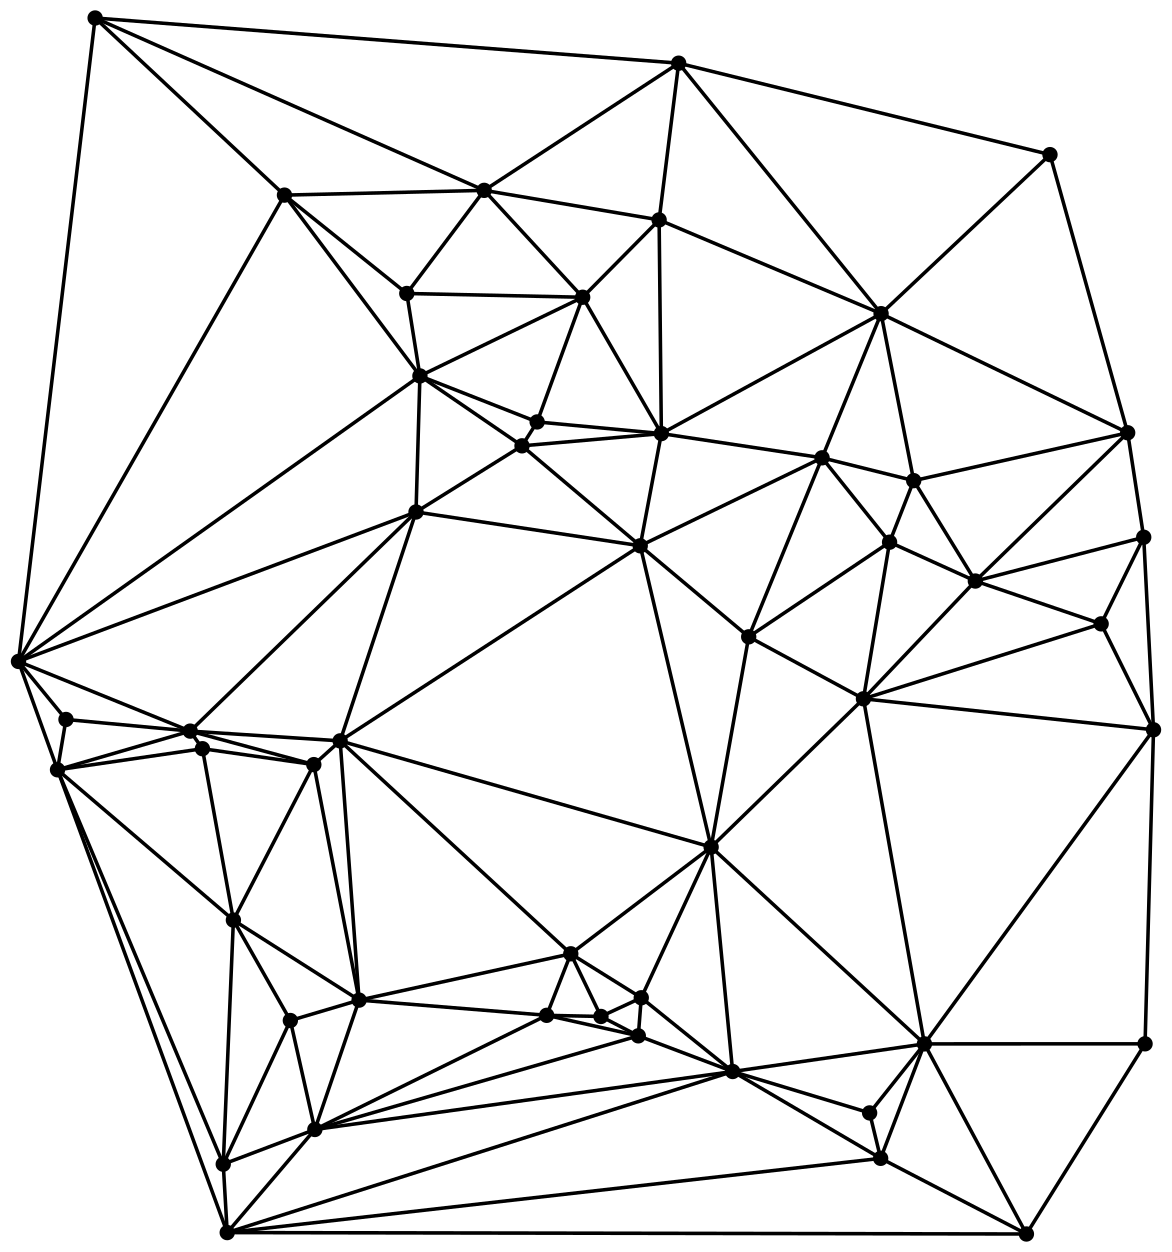
\includegraphics[height=3.3cm]{assets/colon-en/delaunay_mesh.png}\\[2pt]
      {\scriptsize A triangle mesh (Delaunay).\\
       Figure: Inductiveload, \href{https://commons.wikimedia.org/wiki/File:Delaunay_Triangulation_(50_Points).svg}{Wikimedia Commons}, public domain.}
    \end{column}
  \end{columns}
  \TLtakeaway{The whole method reduces to assembling one matrix $\Lmat$ and solving $\Lmat x=b$. The rest of Q4 is: where $\Lmat$ comes from, and solving it by hand on a tiny mesh.}
\end{frame}

% --- 4.2 dirichlet energy bridge --------------------------------------------
\begin{frame}{Least stretch $=$ Dirichlet energy $=$ harmonic}
  ``Keep angles, no spurious wiggle'' is captured by minimizing total stretch --- the \TLterm{Dirichlet energy}:
  \[
    E_D(f)=\half\int_S \nm{\grad f}^2\,\dd A .
  \]
  \begin{itemize}
    \item Its minimizer (with the boundary fixed) is a \TLterm{harmonic} function: $\Lap f=0$. This is the discrete echo of the curvature equation's Laplacian from Q2 --- the Laplacian reappears, now doing the work.
    \item In 2D a \emph{conformal} map's coordinates are harmonic; the exact link is the \href{https://en.wikipedia.org/wiki/Cauchy-Riemann_equations}{Cauchy--Riemann} condition, which needs complex analysis --- taken on faith here, proved in the next deck. So minimizing $E_D$ with a fixed boundary gives harmonic coordinates: angle-preserving \emph{in the conformal limit}, not for an arbitrary boundary.
  \end{itemize}
  \TLtakeaway{We do not need a formula for the map --- we need the field of least stretch. The next two slides turn $E_D$ on a mesh into a matrix, and the cotangent appears on its own.}
\end{frame}

% --- 4.3 PL gradient --------------------------------------------------------
\begin{frame}{One triangle: the gradient of a hat function}
  \begin{columns}[T]
    \begin{column}{0.56\textwidth}
      On a triangle $T=(i,j,k)$, the \textbf{hat function} $\varphi_i$ is linear, equals $1$ at $i$ and $0$ on the opposite edge $jk$.
      \begin{itemize}
        \item Its gradient $\grad\varphi_i$ is \emph{constant} on $T$, points perpendicular to the opposite edge $jk$, with magnitude $1/h_i$, where $h_i$ is the height from $i$ to $jk$.
        \item A piecewise-linear $f=\sum_i f_i\varphi_i$ therefore has constant gradient on each triangle.
      \end{itemize}
      Constant gradients make the energy integral trivial: it is just (area)$\times$(dot product).
    \end{column}
    \begin{column}{0.44\textwidth}
      \centering
      \begin{tikzpicture}[scale=1.1,every node/.style={font=\scriptsize}]
        \coordinate (i) at (0,0); \coordinate (j) at (2.0,0.1); \coordinate (k) at (0.7,1.5);
        \draw[fill=TLprimaryTint] (i)--(j)--(k)--cycle;
        \foreach \p/\l in {i/i,j/j,k/k}{\fill (\p) circle (1.2pt); \node at ($(\p)+(0,0.2)$) {$\l$};}
        \coordinate (foot) at ($(j)!(i)!(k)$);   % foot of perpendicular from i onto edge jk
        \draw[->,TLaccent,very thick] (foot)--(i);
        \node[TLaccent,above left] at ($(foot)!0.5!(i)$) {$\grad\varphi_i$};
        \node[TLneg,below right] at ($(foot)!0.5!(i)$) {$h_i$};
        \node at (1.0,-0.45) {$\grad\varphi_i\perp jk$, toward $i$};
      \end{tikzpicture}
    \end{column}
  \end{columns}
  \TLtakeaway{The only geometric fact we need: $\grad\varphi_i\perp jk$ with length $1/h_i$. From it the cotangent falls out next.}
\end{frame}

% --- 4.4 cotangent appears --------------------------------------------------
\begin{frame}{The cotangent appears (the step worth doing once)}
  Energy needs $\displaystyle\int_T\grad\varphi_i\cdot\grad\varphi_j\,\dd A$. Both gradients are constant, so it is $\text{Area}\cdot(\grad\varphi_i\cdot\grad\varphi_j)$. Let $a=\nm{jk},\,b=\nm{ik}$ and $\theta_k$ the angle at $k$.
  \[
    \grad\varphi_i\perp jk,\ \grad\varphi_j\perp ik\ \Rightarrow\
    \grad\varphi_i\cdot\grad\varphi_j=\frac{\cos(\pi-\theta_k)}{h_i h_j}=-\frac{ab\cos\theta_k}{4\,\text{Area}^2}
    \quad\Big(h_i=\tfrac{2\text{Area}}{a},\,h_j=\tfrac{2\text{Area}}{b}\Big).
  \]
  Multiply by Area, and use $\text{Area}=\half ab\sin\theta_k$:
  \[
    \int_T\grad\varphi_i\cdot\grad\varphi_j\,\dd A=-\frac{ab\cos\theta_k}{4\,\text{Area}}
    =-\frac{ab\cos\theta_k}{2ab\sin\theta_k}=\boxed{-\half\cot\theta_k}.
  \]
  \TLtakeaway{The cotangent is not a convention --- it is $\cos\theta_k/\sin\theta_k$: the $\cos$ from the angle between the two gradients, the $\sin$ from the triangle's area. You just re-derived the heart of the method.}
\end{frame}

% --- 4.5 assemble + Laplacian + signs ---------------------------------------
\begin{frame}{Assemble: the cotangent Laplacian}
  An interior edge $(i,j)$ is shared by two triangles, with \emph{opposite} angles $\alpha_{ij},\beta_{ij}$. Summing both, the energy becomes
  \[
    E_D(f)=\half\sum_{\text{edges }(i,j)} w_{ij}\,(f_i-f_j)^2,\qquad
    \boxed{\,w_{ij}=\half(\cot\alpha_{ij}+\cot\beta_{ij})\,}.
  \]
  \begin{columns}[T]
    \begin{column}{0.6\textwidth}
      Minimizing ($\partial E_D/\partial f_i=0$ at interior vertices) gives the \TLterm{cotangent Laplacian}:
      \[
        (\Lmat f)_i=\sum_{j\sim i} w_{ij}(f_i-f_j)=0 .
      \]
      Entries $L_{ii}=\sum_j w_{ij},\ L_{ij}=-w_{ij}$: symmetric, positive \emph{semi}-definite, \textbf{SPD once the boundary is fixed}.
    \end{column}
    \begin{column}{0.4\textwidth}
      \centering
      \begin{tikzpicture}[scale=0.66,every node/.style={font=\scriptsize}]
        \coordinate (i) at (0,0); \coordinate (j) at (2.1,0.15);
        \coordinate (k) at (1.0,1.4); \coordinate (l) at (1.05,-1.3);
        \draw[fill=TLprimaryTint] (i)--(k)--(j)--cycle;
        \draw[fill=TLprimaryTint] (i)--(l)--(j)--cycle;
        \draw[very thick,TLaccent] (i)--(j);
        \foreach \p/\l in {i/i,j/j,k/k,l/l}{\fill (\p) circle (1.2pt); \node[above] at (\p) {$\l$};}
        \node[TLprimary] at (1.0,1.0) {$\alpha_{ij}$};
        \node[TLprimary] at (1.05,-0.85) {$\beta_{ij}$};
      \end{tikzpicture}\\[1pt]
      {\scriptsize $w_{ij}>0$ when angles aren't too obtuse (Delaunay).}
    \end{column}
  \end{columns}
  \TLtakeaway{``Find the harmonic flattening'' is now literally ``solve $\Lmat x=b$.'' One assembly rule, one sparse SPD solve per coordinate.}
\end{frame}

% --- 4.6 boundary conditions ------------------------------------------------
\begin{frame}{Pin the boundary, solve the interior}
  $\Lmat f=0$ alone has many solutions (constants are harmonic). We make it unique by \textbf{fixing the boundary} --- the rim of the cut-open colon:
  \begin{itemize}
    \item Choose where the boundary loop lands in the plane (a circle or a square).
    \item Hold those boundary vertices fixed; solve $\Lmat x=b$ only for the \emph{interior} vertices, where $b$ collects the pinned boundary terms.
    \item With the boundary fixed, $\Lmat$ (restricted to interior vertices) is SPD $\Rightarrow$ a unique interior layout.
  \end{itemize}
  This is the honest scope from Q3: a \emph{harmonic} map with a chosen boundary --- angle-preserving in the limit, $\approx$ conformal. The boundary choice is the one free decision.
  \TLtakeaway{Boundary fixed $\Rightarrow$ SPD $\Rightarrow$ unique flattening. No existence theorem; just linear algebra. Time to do it by hand.}
\end{frame}

% --- 4.7 worked example -----------------------------------------------------
\begin{frame}{Worked by hand: one interior vertex}
  \begin{columns}[T]
    \begin{column}{0.5\textwidth}
      A regular hexagon fan: six boundary vertices, one interior vertex $c$, six equilateral triangles. Every angle is $60^\circ$, so every spoke weight is equal:
      \[
        w_{ci}=\half(\cot 60^\circ+\cot 60^\circ)=\tfrac{1}{\sqrt3}.
      \]
      Equal weights collapse the interior equation to an average:
      \[
        \sum_{i=1}^{6} w_{ci}(x_c-x_i)=0\ \Rightarrow\ x_c=\tfrac{1}{6}\textstyle\sum_i x_i .
      \]
    \end{column}
    \begin{column}{0.5\textwidth}
      Pin the boundary to a regular hexagon $p_i=(\cos 60^\circ i,\ \sin 60^\circ i)$. Their average is $(0,0)$, so $x_c=(0,0)$, the centroid. Pin an \emph{irregular} hexagon instead and $x_c$ is still the plain average of the six pinned points --- one line of arithmetic.
      \smallskip
      You just ran the whole algorithm in miniature: assemble $\Lmat$ (a $1\times1$ system), impose boundary conditions, solve.
    \end{column}
  \end{columns}
  \TLtakeaway{Harmonic $=$ each free vertex is the cotangent-weighted average of its neighbors. Equal angles give a plain average; unequal angles, a weighted one.}
\end{frame}

% --- 4.8 algorithm summary --------------------------------------------------
\begin{frame}{The algorithm, in five lines}
  \begin{enumerate}
    \item \textbf{Cut} the colon tube open along one curve; you now have a disk with a boundary.
    \item \textbf{Mesh} it into triangles; read off each triangle's angles.
    \item \textbf{Assemble} $\Lmat$ from $w_{ij}=\half(\cot\alpha_{ij}+\cot\beta_{ij})$.
    \item \textbf{Pin} the boundary loop to a circle/square; \textbf{solve} $\Lmat x=b$ for the interior (two coordinates, two SPD solves).
    \item \textbf{Lay} the mesh flat at the solved positions --- the flattened colon.
  \end{enumerate}
  \TLwarnblock{Honest scope}{This is the discrete \emph{harmonic} parametrization. It is angle-preserving in the limit ($\approx$ conformal), not exactly conformal. Making it exact (minimize the Cauchy--Riemann residual / LSCM) is the next deck.}
  \TLtakeaway{Five steps, all linear algebra. The only judgment call is the boundary shape. Now: did it keep its promise, and what did it cost?}
\end{frame}

% =============================================================================
\TLsection{Q5 · Did it work, and what did we pay?}

% --- 5.1 angle check --------------------------------------------------------
\begin{frame}{The promise: angles (measured, not assumed)}
  Check the promise on the flattened mesh: for each triangle compare its three angles before and after the map.
  \begin{itemize}
    \item For the equilateral fan pinned to a regular hexagon, the map is a similarity --- every angle is preserved \emph{exactly}; angle error $=0$.
    \item For a general mesh, the discrete harmonic map preserves angles only \emph{approximately}: small, nonzero residuals. (That gap is precisely what the next deck's exactly-conformal method removes.)
  \end{itemize}
  So we report angle error as a \emph{measured residual} --- near zero, honestly not exactly zero in general.
  \TLtakeaway{The deck does not claim ``angle error $=0$.'' It claims ``small, measured'' --- and tells you exactly which later method drives it to zero.}
\end{frame}

% --- 5.2 area price ---------------------------------------------------------
\begin{frame}{The price: area (an actual number)}
  Area is the bill we agreed to pay in Q3. Measure it directly: for each triangle, the area ratio
  \[
    \text{(area distortion)}_T=\frac{\text{Area}\big(\phi(T)\big)}{\text{Area}(T)} .
  \]
  \begin{itemize}
    \item This per-triangle ratio is the discrete, sampled version of the conformal factor $e^{2u}$ from Q3 --- now a concrete number on each triangle, not a symbol.
    \item Where the original colon bent most (deep folds, high $|K|$), this ratio departs most from $1$: those patches get visibly inflated or shrunk.
  \end{itemize}
  \TLtakeaway{Angles came out near-free; area did not. The histogram of these ratios \emph{is} the bill --- and it is largest exactly where the colon was most curved.}
\end{frame}

% --- 5.3 close the loop -----------------------------------------------------
\begin{frame}{Closing the loop: the bill is the curvature you couldn't remove}
  The area distortion is not bad luck --- it is forced by Q2. The discrete Gauss--Bonnet identity makes it quantitative:
  \[
    \sum_{\text{interior } i}\Big(2\pi-\!\!\sum_{\text{angles at }i}\!\!\theta\Big)=2\pi\chi(S)\quad\text{(total angle deficit}=\text{total curvature)} .
  \]
  \begin{itemize}
    \item A flat layout has \emph{zero} angle deficit at interior vertices. The colon's deficit is nonzero (its curvature, from Q2).
    \item That mismatch cannot be destroyed --- only \emph{moved} into the one channel we left open: area. So nonzero curvature in Q2 \emph{guarantees} nonzero area distortion in Q5.
  \end{itemize}
  \TLtakeaway{The number you measured in Q5 was inevitable the moment Q2 proved $K\neq0$. The deck closes its own loop: the price equals the curvature you were never allowed to remove.}
\end{frame}

% --- 5.4 clinical reading ---------------------------------------------------
\begin{frame}{Reading the flattened colon (the honest user's guide)}
  \begin{columns}[T]
    \begin{column}{0.5\textwidth}
      \TLinfoblock{Trust}{Local \emph{shape}. A polyp stays round; folds keep their angular structure. Shape-based detection works on the flat image.}
    \end{column}
    \begin{column}{0.5\textwidth}
      \TLwarnblock{Distrust}{Absolute \emph{size}, especially near deep folds where the area ratio is far from $1$. Read sizes against the area-distortion map, not at face value.}
    \end{column}
  \end{columns}
  \medskip
  That is the whole trade, stated plainly: we gave up length (forced), kept angle (chosen, for shape), and pay in area (measured, and bounded below by curvature).
  \TLtakeaway{A good flattening is not distortion-free --- it is one whose single distortion is \emph{known, located, and explained.} That is what we built.}
\end{frame}

% =============================================================================
\TLsection{What we built · what's next · notation · exercises · references}

% --- synthesis / next decks -------------------------------------------------
\begin{frame}{What we built, and the next decks}
  \begin{columns}[T]
    \begin{column}{0.56\textwidth}
      \textbf{This deck, end to end:}
      \begin{itemize}
        \item Why no distortion-free flattening exists (Theorema Egregium, proven impossibility).
        \item Why we keep angles (clinical), and what that costs (area $=e^{2u}$).
        \item One method, fully built and hand-solved: the cotangent Laplacian, harmonic map, fixed boundary.
      \end{itemize}
    \end{column}
    \begin{column}{0.44\textwidth}
      \textbf{Next decks (each built to this depth):}
      \begin{itemize}
        \item \emph{Exactly} conformal: minimize the Cauchy--Riemann residual (LSCM).
        \item Global structure: holomorphic 1-forms / Hodge theory.
        \item Programmable target curvature: Ricci flow.
      \end{itemize}
    \end{column}
  \end{columns}
  \TLtakeaway{One question, one method, fully owned --- the template for the series. Each later deck removes one of this deck's honest limitations.}
\end{frame}

% --- notation ---------------------------------------------------------------
\begin{frame}{Notation (only what we used)}
  \begin{columns}[T]
    \begin{column}{0.5\textwidth}
      \begin{tabular}{@{}ll@{}}
        $\xb(u,v)$ & surface as a map into $\R^3$\\
        $\xb_u,\xb_v$ & tangent vectors (the rulers)\\
        $E,F,G$ & first fundamental form (metric)\\
        $\kappa_1,\kappa_2$ & principal curvatures\\
        $K=\kappa_1\kappa_2$ & Gauss curvature\\
      \end{tabular}
    \end{column}
    \begin{column}{0.5\textwidth}
      \begin{tabular}{@{}ll@{}}
        $e^{2u}$ & conformal factor (area price)\\
        $\varphi_i$ & hat function at vertex $i$\\
        $\alpha_{ij},\beta_{ij}$ & angles opposite edge $(i,j)$\\
        $w_{ij}$ & cotangent weight\\
        $\Lmat$ & cotangent Laplacian ($\Lmat x=b$)\\
      \end{tabular}
    \end{column}
  \end{columns}
  \TLtakeaway{Ten symbols, each introduced where a question needed it. If you can define all ten from memory, you can re-derive the deck.}
\end{frame}

% --- exercises --------------------------------------------------------------
\begin{frame}{Exercises (do these, then you own it)}
  \begin{enumerate}
    \item \textbf{Metric}: compute $E,F,G$ for the cylinder $\xb=(r\cos u,r\sin u,v)$ and confirm a rescaling makes it the flat metric.
    \item \textbf{Curvature}: from the sphere's principal curvatures, confirm $K=1/R^2$; explain in one line why the cylinder's $K=0$.
    \item \textbf{Cotangent}: for a $45^\circ$--$45^\circ$--$90^\circ$ triangle, compute the weight contribution $-\half\cot\theta_k$ for each angle.
    \item \textbf{Solve}: take the one-interior-vertex fan, pin the boundary to an \emph{irregular} hexagon of your choice, and solve for the interior vertex (it is the weighted average --- get a number).
    \item \textbf{Loop}: argue from discrete Gauss--Bonnet why a colon with $K\neq0$ \emph{must} show nonzero area distortion after any flat layout.
  \end{enumerate}
\end{frame}

% --- references -------------------------------------------------------------
\begin{frame}{References \& figure credits}
  \footnotesize
  \begin{thebibliography}{9}
    \setbeamertemplate{bibliography item}[text]
    \bibitem{docarmo} M.~do Carmo. \emph{Differential Geometry of Curves and Surfaces}. Prentice-Hall, 1976. (metric, curvature, Theorema Egregium --- \S2--\S4)
    \bibitem{egregium} \href{https://en.wikipedia.org/wiki/Theorema_Egregium}{Theorema Egregium} and \href{https://en.wikipedia.org/wiki/Gaussian_curvature}{Gaussian curvature} (Wikipedia) --- full statements and the Brioschi proof.
    \bibitem{uniform} \href{https://en.wikipedia.org/wiki/Uniformization_theorem}{Uniformization theorem} (Wikipedia) --- smooth conformal existence, cited not proven.
    \bibitem{cotan} \href{https://en.wikipedia.org/wiki/Discrete_Laplace_operator}{Discrete Laplace operator} (Wikipedia) --- the cotangent weights on a mesh.
    \bibitem{hat} S.~Haker, S.~Angenent, A.~Tannenbaum, R.~Kikinis. \emph{Nondistorting flattening maps and the 3D visualization of colon CT images}. IEEE TMI, 19(7), 2000. (harmonic colon flattening)
  \end{thebibliography}
  \smallskip
  {\scriptsize Figure credits (all openly licensed, via Wikimedia Commons): Gaussian-curvature surfaces --- Nicoguaro, CC0; colon anatomy --- Mikael Häggström, public domain; conformal map --- Oleg Alexandrov, public domain; triangle mesh --- Inductiveload, public domain. All other figures original (TikZ).}
\end{frame}

\end{document}
